%!TeX program = xelatex
\PassOptionsToPackage{quiet}{fontspec}
\documentclass[10.5pt,compsoc,UTF8]{CjC}
\usepackage{thesis}
%===============================%信息设置
\mycourse{《高等物理海洋学》}
\mytitle{安达曼海内孤立波特征分析}
\myauthor{陈鹏亦}
\mystudentid{22434197}
\myschool{海洋学院}
\myteacher{宋金宝}

\begin{document}
\setpage

\Title{\themytitle}{\themyauthor}{\themystudentid}

\myabstract{

}
\vspace {5mm}
\keyword{摸鱼;LaTeX}


\vskip 45mm

\begin{center}
\zihao{3}{ \bf LaTeX on Overleaf}\\
\vspace {5mm}

\end{center}

\zihao{5}{\noindent
{\bf Abstract}\quad 
\zihao{5}{\noindent \lipsum[5]
\par}}
\vspace {5mm}
{\noindent{\bf Keywords}\quad LaTeX}


% 正文
\clearpage
\section{引言}
内波是一种发生在密度稳定层化的海洋内的波动\cite{Liang2016}。
与表面波不同,内波引起的近海表面的等密度面垂向起伏通常很小,其最大振幅往往出现在海洋内部\cite{}。
海洋中内波主要有三种:一种是由于风引起的,在海洋混合层内激发的波动频率接近于惯性频率的内波\cite{};
一类是由于正压潮流经过海底变化地形时产生的内潮波;还有一类是内潮波经过非线性增强得到的内孤立波\cite{}。
本文主要对安达曼海内孤立波的特征进行分析。

安达曼海位于印度洋东北部(经纬度范围:$ 93 - 100^\circ E $、$ 6 - 14^\circ N $),是印度洋的一个次海域,北界为孟加拉湾,东界为泰国半岛,南界为尼科巴群岛,西界为安达曼群岛\cite{}。
安达曼海地形及内孤立波生成源地如图 \ref{fig:1} 所示。
% 单图
\begin{figure}[!htbp]
    \centering
    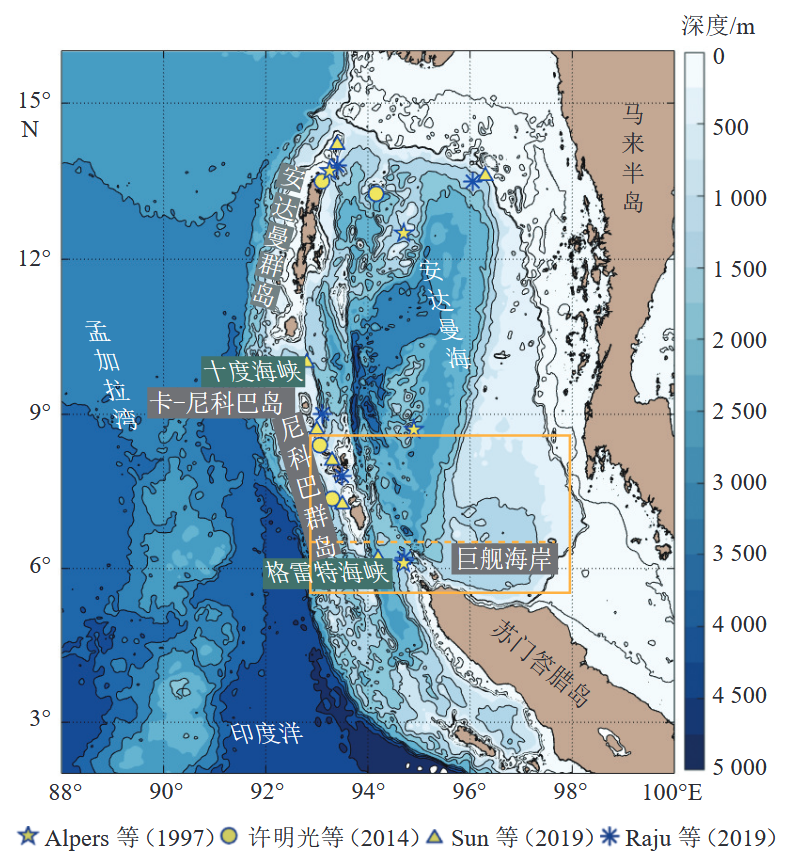
\includegraphics[width=0.8\textwidth]{fig1.png}
    \caption{安达曼海地形及内孤立波生成源地(注:4种标记为不同文献中确定的安达曼海内孤立波的生成源地。图源:\cite{Zhang2024})}
    \label{fig:1}
\end{figure}

% \begin{table}[htbp]
%   \centering
%     \begin{tabular}{ccp{20em}}
%     \toprule
%     编号    & 仪器用具名称     & 主要参数(型号,测量范围,测量精度等) \\
%     \midrule
%     1	&	数字万用表\\
%     2	&	直流稳压电源\\
%     3	&	电子技术实验箱\\
%     4	&	示波器\\
%     5	&	函数信号发生器\\
%         6   &	运放LM358\\
%     \bottomrule
%     \end{tabular}%
%   \label{tab:device}%
%   \caption{我是一个表格}
% \end{table}%

\section{实测数据}
安达曼海的内波观测最早可追溯到1964年6月美国海岸和大地测量船Pioneer号在苏门答腊岛北部和与尼科巴海脊之间的观测,这次观测得到了至少5个内孤立波活动区域,观测到的内孤立波最大振幅可达82m。
随后Osborne等人,在安达曼海
\begin{figure}[!htbp]
    \centering
    \begin{minipage}[b]{0.45\linewidth}
        \centering
        \includegraphics[width=0.9\textwidth]{example}
        \caption{非子图并排题注1}
         
    \end{minipage}%
    \begin{minipage}[b]{0.45\linewidth}
        \centering
        \includegraphics[width=0.9\textwidth]{example}
        \caption{非子图并排题注2}
         
    \end{minipage}
\end{figure}


\section{第二节}


\zhlipsum[5] % 生成随机文字

杭州不要再下雨啦,我知道你有你的烦恼,但我们也期盼着能有更多的阳光洒满这座美丽的城市。虽然雨水能带来生机和活力,但持续的阴雨天气也会让人感到压抑和沉闷。让我们一起期待阳光的到来,让杭州的天空重新焕发出明亮的光彩。同时,也希望大家在雨天注意出行安全,照顾好自己和身边的人。

\begin{figure}
    \centering
    \includegraphics[width=0.5\linewidth]{figures/example.png}
    \caption{Enter Caption}
    \label{fig:enter-label}
\end{figure}


\newpage
\section{代码展示}
\begin{problem}
adsfa
\end{problem}
\begin{solution}
\end{solution}
\begin{lstlisting}[language=Python, caption=Python example]
def hello_world():
    print("Hello, world!")
\end{lstlisting}


% 参考文献
\clearpage
\reference
\end{document}


